%% Short communication prepared with the Elsevier article class
%% (elsarticle.cls, https://ctan.org/pkg/elsarticle).
%% Target journal: Digital Chemical Engineering.
\documentclass[preprint,12pt]{elsarticle}

\usepackage[utf8]{inputenc}
\usepackage[T1]{fontenc}
\usepackage{lmodern}
\usepackage{amsmath}
\usepackage{booktabs}
\usepackage{tabularx}
\usepackage{graphicx}
\usepackage{tikz}
\usetikzlibrary{arrows.meta,positioning,fit}
\usepackage{xurl}
\usepackage{hyperref}

\journal{Digital Chemical Engineering}

\begin{document}

\begin{frontmatter}

\title{Formats carry, ontologies anchor: FAIR exchange of enzyme kinetics
and process flowsheets between EnzymeML, DEXPI and BioSTEAM}

%% TODO (authors): complete names, affiliations and corresponding author.
\author[inst1]{First Author\corref{cor1}}
\ead{corresponding.author@example.org}
\author[inst1]{Second Author}
\cortext[cor1]{Corresponding author.}
\affiliation[inst1]{organization={Department, Institution},
            city={City},
            country={Country}}

\begin{abstract}
Reusing laboratory kinetics in process simulation still means retyping
numbers, because the data leave the laboratory and the flowsheet leaves the
engineering tool in forms the simulator cannot read. Earlier work bridged
this gap with a dedicated ontology and knowledge graph. We ask whether such
an ontology is required, or whether widely used exchange formats suffice
once they refer to maintained vocabularies. We connected an EnzymeML
document and a DEXPI~2.0 process model to the open-source simulator BioSTEAM
using only the two formats and the identifiers they already carry. For the
regeneration of NADH by formate dehydrogenase in a stirred tank, kinetics
and flowsheet combined into a running simulation without manual
transcription, and an export to DEXPI followed by re-import reproduced all
stream results. Everything that was anchored to a shared identifier or an
enumerated vocabulary transferred automatically; everything that was only
named locally needed a convention or a human. We conclude that formats and
ontologies are complementary: formats are what tools implement, ontologies
are what make their content unambiguous, and the maintained mapping between
the two is the scarce resource.
\end{abstract}

\begin{highlights}
\item EnzymeML kinetics and a DEXPI flowsheet run in BioSTEAM without
      transcription.
\item A DEXPI export and re-import reproduces all simulated stream results.
\item Content with shared identifiers transfers automatically; local names
      do not.
\item Exchange formats and ontologies are complementary, not alternatives.
\item Maintained format-to-ontology mappings are the missing piece for
      reuse.
\end{highlights}

\begin{keyword}
FAIR data \sep interoperability \sep ontology \sep DEXPI \sep EnzymeML
\sep process simulation \sep biocatalysis
\end{keyword}

\end{frontmatter}

\section{Introduction}

The FAIR principles ask that data be findable, accessible, interoperable
and reusable~\cite{wilkinson2016}. In bioprocess development the last two
are the hard ones. Kinetic parameters are measured in the laboratory, the
process is drawn in an engineering tool, and the simulation is set up in a
third program, usually by typing the first two into it.

Behr et al.~\cite{behr2024} showed that this chain can be partly automated.
They recorded enzyme kinetics with EnzymeML~\cite{lauterbach2023},
represented them with concepts from ontologies in a knowledge graph, and
generated a simulation in the open-source simulator DWSIM from that graph.
Their work places the ontology at the centre of the data flow.

This raises a practical question for anyone building such a pipeline. FAIR
principle~I1 calls for a formal, shared and broadly applicable language,
I2 for vocabularies that are themselves FAIR, and R1.3 for adherence to
community standards~\cite{wilkinson2016}. An ontology answers I2; a
community exchange format answers R1.3; and it is not obvious which of the
two a pipeline should be built around. Ontologies give terms a meaning
that does not depend on the tool that wrote them~\cite{guizzardi2020}, but
few engineering tools read or write them. Exchange formats are implemented
by many tools, but a format alone fixes structure, not meaning.

Here we test the second route. We connect EnzymeML and the process part of
DEXPI~2.0, which covers block and process flow
diagrams~\cite{cameron2024}, to BioSTEAM~\cite{cortespena2020} using
nothing but the two formats and the identifiers they contain, and we record
where that was enough and where it was not.

\section{Methods}

\subsection{Implementation}

We extended BioSTEAM with three modules (Fig.~\ref{fig:workflow}). The
first reads and writes DEXPI~2.0 XML and translates between process steps
and unit operations through a registry that follows the class hierarchy of
the specification. The second reads EnzymeML version~2 JSON and turns a
reaction, its rate law and its parameters into a kinetic reaction. The
third resolves chemical identities (CAS number, InChIKey, ChEBI and PubChem
identifiers) to property data, trying user data first, then the simulator's
databases, optionally PubChem, and finally a placeholder with water-like
properties that is reported to the user.

Both readers use only the Python standard library. We wrote the DEXPI
adapter against the specification rather than building on
pyDEXPI~\cite{pydexpi}, whose AGPL licence is incompatible with the
permissive licence of BioSTEAM; pyDEXPI serves as an independent
conformance check in the test suite. The EnzymeML Python
library~\cite{pyenzyme} is optional and only needed for archive files.

BioSTEAM evaluates a kinetic reaction as a rate for a given stream. For a
continuous stirred tank we therefore solve the steady-state balance
\begin{equation}
  \xi = r\bigl(C_\mathrm{out}(\xi)\bigr)\,V, \qquad
  C_{\mathrm{out},i} = \frac{F_i + \nu_i\,\xi}{Q}, \qquad V = \tau Q,
\end{equation}
for the conversion $\xi$, with rate law $r$, feed flows $F_i$,
stoichiometric numbers $\nu_i$, volumetric flow $Q$ and residence time
$\tau$. Rate laws arrive as text and are evaluated by a parser that accepts
arithmetic only. Parameters are converted with the unit definitions of the
EnzymeML document.

DEXPI has no attributes for simulator-specific settings such as residence
time or kinetics. On export we store them as JSON in standard DEXPI
\texttt{Note} objects, so that the file remains valid for other tools.

\begin{figure}[t]
\centering
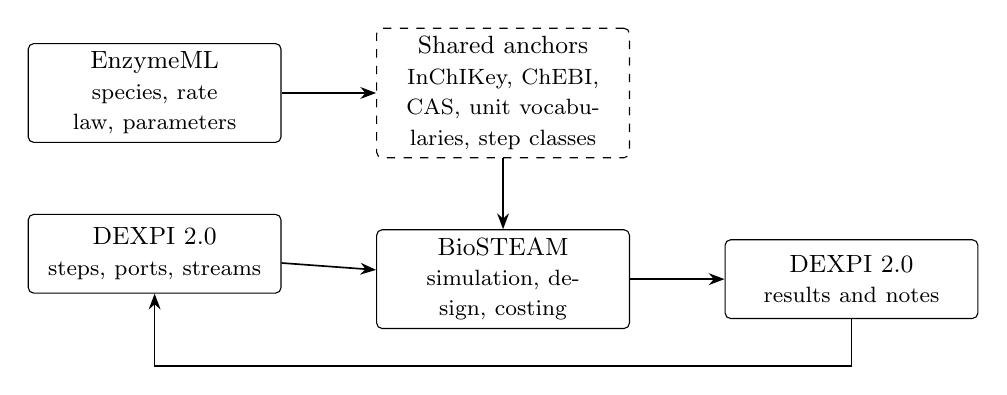
\begin{tikzpicture}[
    font=\small,
    box/.style={draw, rounded corners=2pt, align=center, minimum height=10mm,
                text width=30mm, inner sep=3pt},
    anchorbox/.style={draw, dashed, rounded corners=2pt, align=center,
                text width=30mm, inner sep=3pt},
    arr/.style={-{Stealth[length=2mm]}, semithick},
    node distance=9mm and 12mm]
  \node[box] (eml) {EnzymeML\\{\footnotesize species, rate law, parameters}};
  \node[box, below=of eml] (dexpi) {DEXPI 2.0\\{\footnotesize steps, ports, streams}};
  \node[anchorbox, right=of eml] (ids) {Shared anchors\\{\footnotesize InChIKey, ChEBI, CAS, unit vocabularies, step classes}};
  \node[box, below=of ids] (bst) {BioSTEAM\\{\footnotesize simulation, design, costing}};
  \node[box, right=of bst] (out) {DEXPI 2.0\\{\footnotesize results and notes}};
  \draw[arr] (eml) -- (ids);
  \draw[arr] (dexpi) -- (bst);
  \draw[arr] (ids) -- (bst);
  \draw[arr] (bst) -- (out);
  \draw[arr] (out.south) -- ++(0,-6mm) -| (dexpi.south);
\end{tikzpicture}
\caption{Data flow. Kinetics and flowsheet enter as community exchange
formats; shared identifiers and vocabularies (dashed) align their content.
The simulated system is exported as DEXPI and can be imported again.}
\label{fig:workflow}
\end{figure}

\subsection{Reference case}

The case is the regeneration of NADH by formate dehydrogenase (FDH,
EC~1.17.1.9), with formate as sacrificial cosubstrate:
\begin{equation}
  \text{formate} + \text{NAD}^+ \longrightarrow \text{CO}_2 + \text{NADH}.
\end{equation}
The EnzymeML document holds the initial-rate form of an ordered bi-bi rate
law with four parameters
($k_\mathrm{cat} = 3.7~\mathrm{s^{-1}}$,
$K_{\mathrm{m,formate}} = 5.6~\mathrm{mM}$,
$K_{\mathrm{m,NAD}} = 0.045~\mathrm{mM}$,
$K_{\mathrm{i,NAD}} = 0.04~\mathrm{mM}$).
These are representative values chosen to exercise the workflow, not a
curated measurement. The DEXPI file describes a feed, a pump and a reactor
at $30~^{\circ}\mathrm{C}$; it was written without any BioSTEAM-specific
content and in units that differ from those of the simulator
($^{\circ}$C, bar, kmol~s$^{-1}$). The feed contains about
$100~\mathrm{mol~m^{-3}}$ formate, $5~\mathrm{mol~m^{-3}}$ NAD$^+$ and
$0.2~\mathrm{mmol~m^{-3}}$ enzyme in water at $1~\mathrm{m^3~h^{-1}}$.

\section{Results}

\subsection{From two files to a simulation}

Reading the two files and assigning the reaction to the reactor produced a
running model in a handful of function calls. At a residence time of $2~\mathrm{h}$ the
simulation gave 90.4\% conversion of NAD$^+$ in a reactor of
$2.5~\mathrm{m^3}$. No number was transcribed by hand; the only inputs
beyond the two files were the residence time, the formula of NADH and the
molecular weight of the enzyme.

\subsection{Round trip}

We exported the simulated system to DEXPI and imported it into a separate
flowsheet with a property package rebuilt from the identifiers in the
file. Simulating the imported system reproduced the molar flows of every
stream, the reactor volume, the heat duty and the installed equipment cost
to within a relative difference of $10^{-9}$, also when export and import
ran in two separate Python processes that shared only the file. The same
held for a seven-unit flowsheet with a recycle when both systems were
simulated from the same starting point. Exported files load in the strict
mode of pyDEXPI, and a file written by pyDEXPI imports into BioSTEAM.

\subsection{What transferred, and what did not}

Table~\ref{tab:anchors} sorts the content of the two files by how it was
identified. The pattern is consistent. Content tied to a shared identifier
or an enumerated vocabulary crossed the tool boundary without help. Content
that was only named locally did not.

\begin{table}[t]
\caption{Content of the exchanged files, how it is identified, and whether
it transferred without human input.}
\label{tab:anchors}
\small
\begin{tabularx}{\textwidth}{@{}>{\raggedright\arraybackslash}p{33mm}
    >{\raggedright\arraybackslash}X
    >{\raggedright\arraybackslash}p{36mm}@{}}
\toprule
Content & Identified by & Transfer \\
\midrule
Small molecules & InChIKey, ChEBI, CAS & Automatic \\
Units of measurement & Enumerated unit literals (DEXPI); unit definitions
  (EnzymeML) & Automatic \\
Unit operation type & DEXPI process step class and its parent classes &
  Automatic; unknown classes kept as placeholders \\
Topology & Port and stream references & Automatic \\
Species in rate law vs.\ flowsheet component & Local names in each file &
  Convention: equal names, or a rename table \\
Enzyme & EC number, organism; no molecular weight & Manual \\
NADH properties & ChEBI; absent from property database & Manual (formula) \\
Kinetics in the flowsheet & No DEXPI attribute & Free-text note (JSON) \\
Meaning of rate-law symbols & Implicit & Convention \\
\bottomrule
\end{tabularx}
\end{table}

Three observations deserve a remark. First, the class hierarchy of DEXPI
did useful semantic work: a step of a class the simulator has no model for
is interpreted through its parent class, and where none applies the
topology is kept with a placeholder that restores the original class on
export. Second, a precise identifier is not automatically the right one.
The reaction is written with formate (CHEBI:15740), but the mass balance
only closes in atoms with formic acid (CHEBI:30751), which is what a
property database provides; choosing between them is a modelling decision
that no identifier makes for the user. Third, the kinetics survive the
round trip only because we placed them in a note. Another DEXPI tool will
display that note but cannot interpret it.

\section{Discussion}

\subsection{Are ontologies the key?}

Our pipeline contains no ontology file, no reasoner and no knowledge
graph, and it reproduces the kind of transfer that motivated the
ontology-centred approach~\cite{behr2024}. It would be wrong to conclude
that ontologies are unnecessary. Every row of Table~\ref{tab:anchors}
marked automatic rests on one: ChEBI is an ontology of chemical
entities~\cite{hastings2016}, the process step classes of DEXPI form a
taxonomy, and the unit literals are a controlled vocabulary. The formats
succeeded where they point to such resources and failed where they do
not. This is the role Guizzardi assigns to ontologies in FAIR: they are
the contract about what a term means~\cite{guizzardi2020}.

What the experiment does show is that the ontology need not be the
exchange medium. A tool developer implements a reader for a format that
many other tools write. Systems biology took this path with
SBML~\cite{hucka2003}, on which the first version of EnzymeML
builds~\cite{lauterbach2023}. Both formats used here already provide the
hooks. EnzymeML version~2 is serialised as JSON-LD, whose context maps its
fields to terms of schema.org, OBO ontologies and unit ontologies. DEXPI
gives pure components ChEBI and IUPAC identifiers and lets a value carry a
reference-data URI. The semantic layer is thus present in the files; it is
thin, and it is uneven.

\subsection{Both, joined by maintained mappings}

We therefore answer the question in the title of this section with
``both'', and add a condition. Formats that are widely implemented make
data \emph{reach} the next tool. References to maintained ontologies make
the data \emph{mean} the same thing there. What is missing in practice is
the mapping between the two, kept current as both sides evolve.

The rows of Table~\ref{tab:anchors} that needed a convention or a human
are a list of such missing mappings: no shared term links an EnzymeML
species to a DEXPI material component, a DEXPI reactor has no standard way
to refer to a rate law, and the meaning of a rate-law symbol is not
stated. Process engineering ontologies such as
OntoCAPE~\cite{morbach2007} and the chemistry ontologies surveyed
in~\cite{stroemert2022} contain suitable concepts. Publishing mappings
from format elements to those concepts in a machine-readable form such as
SSSOM~\cite{matentzoglu2022} would let each tool keep its simple reader
while gaining the cross-domain meaning that a knowledge graph provides.
In this view the knowledge graph of Behr et al.\ and the format-based
route are two renderings of the same information, and a mapping makes
them interchangeable.

Reuse also has a non-semantic side. The FAIR principles for research
software ask for clear licences and for software that can be built upon
\cite{barker2022}. The need to re-implement a format because the reference
library carries a copyleft licence is a reminder that interoperability
can fail on terms of use before it fails on terms of meaning.

\subsection{Limitations}

This is one reaction in one reactor with illustrative parameters. We did
not score the result against formal FAIR metrics, and we did not test
reasoning over an ontology, which is where the ontology-centred approach
may show advantages our comparison cannot. The kinetics are isothermal,
enzyme and cofactor properties are estimates that affect energy but not
mass balances, and energy streams of DEXPI are not yet translated.

\section{Conclusions}

Laboratory kinetics in EnzymeML and a flowsheet in DEXPI can be combined
into a process simulation, and exchanged again, using the formats alone.
Where the files refer to shared identifiers and vocabularies the transfer
is automatic; where they use local names it depends on convention. Formats
and ontologies are therefore not competing answers to FAIR
interoperability. Community formats should remain the carrier, ontologies
the reference, and the community's effort is best spent on maintained
mappings between them, starting with the link between a kinetic model and
the reactor it describes.

\section*{CRediT authorship contribution statement}
%% TODO (authors): complete according to actual contributions.
\textbf{First Author:} Conceptualization, Methodology, Software, Writing --
original draft. \textbf{Second Author:} Supervision, Writing -- review \&
editing.

\section*{Declaration of competing interest}
The authors declare that they have no known competing financial interests
or personal relationships that could have appeared to influence the work
reported in this paper.

\section*{Data availability}
The implementation, the EnzymeML document, the DEXPI process model, a
tutorial notebook and the tests that produce every number reported here
are available in the development branch of the repository at
\url{https://github.com/NMEpping/biosteam/tree/claude/biosteam-dexpi-interop-7v0748}.
%% TODO (authors): archive a release and cite its DOI.

\section*{Declaration of generative AI and AI-assisted technologies in the
writing process}
During the preparation of this work the authors used Claude (Anthropic) to
develop the software and to draft the manuscript. After using this tool,
the authors reviewed and edited the content as needed and take full
responsibility for the content of the published article.

\section*{Acknowledgements}
%% TODO (authors): funding and acknowledgements.
This research did not receive any specific grant from funding agencies in
the public, commercial, or not-for-profit sectors.

\bibliographystyle{elsarticle-num}
\bibliography{references}

\end{document}
